% Options for packages loaded elsewhere
\PassOptionsToPackage{unicode}{hyperref}
\PassOptionsToPackage{hyphens}{url}
%
\documentclass[
  ignorenonframetext,
]{beamer}
\usepackage{pgfpages}
\setbeamertemplate{caption}[numbered]
\setbeamertemplate{caption label separator}{: }
\setbeamercolor{caption name}{fg=normal text.fg}
\beamertemplatenavigationsymbolsempty
% Prevent slide breaks in the middle of a paragraph
\widowpenalties 1 10000
\raggedbottom
\setbeamertemplate{part page}{
  \centering
  \begin{beamercolorbox}[sep=16pt,center]{part title}
    \usebeamerfont{part title}\insertpart\par
  \end{beamercolorbox}
}
\setbeamertemplate{section page}{
  \centering
  \begin{beamercolorbox}[sep=12pt,center]{part title}
    \usebeamerfont{section title}\insertsection\par
  \end{beamercolorbox}
}
\setbeamertemplate{subsection page}{
  \centering
  \begin{beamercolorbox}[sep=8pt,center]{part title}
    \usebeamerfont{subsection title}\insertsubsection\par
  \end{beamercolorbox}
}
\AtBeginPart{
  \frame{\partpage}
}
\AtBeginSection{
  \ifbibliography
  \else
    \frame{\sectionpage}
  \fi
}
\AtBeginSubsection{
  \frame{\subsectionpage}
}
\usepackage{amsmath,amssymb}
\usepackage{lmodern}
\usepackage{ifxetex,ifluatex}
\ifnum 0\ifxetex 1\fi\ifluatex 1\fi=0 % if pdftex
  \usepackage[T1]{fontenc}
  \usepackage[utf8]{inputenc}
  \usepackage{textcomp} % provide euro and other symbols
\else % if luatex or xetex
  \usepackage{unicode-math}
  \defaultfontfeatures{Scale=MatchLowercase}
  \defaultfontfeatures[\rmfamily]{Ligatures=TeX,Scale=1}
  \setmainfont[BoldFont = SF Pro Rounded Semibold]{SF Pro Rounded}
  \setmathfont[]{STIX Two Math}
\fi
\usefonttheme{serif} % use mainfont rather than sansfont for slide text
% Use upquote if available, for straight quotes in verbatim environments
\IfFileExists{upquote.sty}{\usepackage{upquote}}{}
\IfFileExists{microtype.sty}{% use microtype if available
  \usepackage[]{microtype}
  \UseMicrotypeSet[protrusion]{basicmath} % disable protrusion for tt fonts
}{}
\makeatletter
\@ifundefined{KOMAClassName}{% if non-KOMA class
  \IfFileExists{parskip.sty}{%
    \usepackage{parskip}
  }{% else
    \setlength{\parindent}{0pt}
    \setlength{\parskip}{6pt plus 2pt minus 1pt}}
}{% if KOMA class
  \KOMAoptions{parskip=half}}
\makeatother
\usepackage{xcolor}
\IfFileExists{xurl.sty}{\usepackage{xurl}}{} % add URL line breaks if available
\IfFileExists{bookmark.sty}{\usepackage{bookmark}}{\usepackage{hyperref}}
\hypersetup{
  pdftitle={305 Lecture 7.3 - Inverting Conditional Probability},
  pdfauthor={Brian Weatherson},
  hidelinks,
  pdfcreator={LaTeX via pandoc}}
\urlstyle{same} % disable monospaced font for URLs
\newif\ifbibliography
\usepackage{longtable,booktabs,array}
\usepackage{calc} % for calculating minipage widths
\usepackage{caption}
% Make caption package work with longtable
\makeatletter
\def\fnum@table{\tablename~\thetable}
\makeatother
\usepackage{graphicx}
\makeatletter
\def\maxwidth{\ifdim\Gin@nat@width>\linewidth\linewidth\else\Gin@nat@width\fi}
\def\maxheight{\ifdim\Gin@nat@height>\textheight\textheight\else\Gin@nat@height\fi}
\makeatother
% Scale images if necessary, so that they will not overflow the page
% margins by default, and it is still possible to overwrite the defaults
% using explicit options in \includegraphics[width, height, ...]{}
\setkeys{Gin}{width=\maxwidth,height=\maxheight,keepaspectratio}
% Set default figure placement to htbp
\makeatletter
\def\fps@figure{htbp}
\makeatother
\setlength{\emergencystretch}{3em} % prevent overfull lines
\providecommand{\tightlist}{%
  \setlength{\itemsep}{0pt}\setlength{\parskip}{0pt}}
\setcounter{secnumdepth}{-\maxdimen} % remove section numbering
\let\Tiny=\tiny

 \setbeamertemplate{navigation symbols}{} 

% \usetheme{Madrid}
 \usetheme[numbering=none, progressbar=foot]{metropolis}
 \usecolortheme{wolverine}
 \usepackage{color}
 \usepackage{MnSymbol}
% \usepackage{movie15}

\usepackage{amssymb}% http://ctan.org/pkg/amssymb
\usepackage{pifont}% http://ctan.org/pkg/pifont
\newcommand{\cmark}{\ding{51}}%
\newcommand{\xmark}{\ding{55}}%

\DeclareSymbolFont{symbolsC}{U}{txsyc}{m}{n}
\DeclareMathSymbol{\boxright}{\mathrel}{symbolsC}{128}
\DeclareMathAlphabet{\mathpzc}{OT1}{pzc}{m}{it}

\usepackage{tikz-qtree}
% \usepackage{markdown}
%\RequirePackage{bussproofs}
\usetikzlibrary{arrows.meta}
\RequirePackage[tableaux]{prooftrees}
\forestset{line numbering, close with = x}
% Allow for easy commas inside trees
\renewcommand{\,}{\text{, }}


\usepackage{tabulary}

\usepackage{open-logic-config}

\setlength{\parskip}{1ex plus 0.5ex minus 0.2ex}

\AtBeginSection[]
{
\begin{frame}
	\Huge{\color{darkblue} \insertsection}
\end{frame}
}

\renewenvironment*{quote}	
	{\list{}{\rightmargin   \leftmargin} \item } 	
	{\endlist }

\definecolor{darkgreen}{rgb}{0,0.7,0}
\definecolor{darkblue}{rgb}{0,0,0.8}

\newcommand{\starttab}{\begin{center}
\vspace{6pt}
\begin{tabular}}

\newcommand{\stoptab}{\end{tabular}
\vspace{6pt}
\end{center}
\noindent}


\newcommand{\sif}{\rightarrow}
\newcommand{\siff}{\leftrightarrow}
\newcommand{\EF}{\end{frame}}


\newcommand{\TreeStart}[1]{
%\end{frame}
\begin{frame}
\begin{center}
\begin{tikzpicture}[scale=#1]
\tikzset{every tree node/.style={align=center,anchor=north}}
%\Tree
}

\newcommand{\TreeEnd}{
\end{tikzpicture}
%\end{center}
}

\newcommand{\DisplayArg}[2]{
\begin{enumerate}
{#1}
\end{enumerate}
\vspace{-6pt}
\hrulefill

%\hspace{14pt} #2
%{\addtolength{\leftskip}{14pt} #2}
\begin{quote}
{\normalfont #2}
\end{quote}
\vspace{12pt}
}

\newenvironment{ProofTree}[1][1]{
\begin{center}
\begin{tikzpicture}[scale=#1]
\tikzset{every tree node/.style={align=center,anchor=south}}
}
{
\end{tikzpicture}
\end{center}
}

\newcommand{\TreeFrame}[2]{
\begin{columns}[c]
\column{0.5\textwidth}
\begin{center}
\begin{prooftree}{}
#1
\end{prooftree}
\end{center}
\column{0.45\textwidth}
%\begin{markdown}
#2
%\end{markdown}
\end{columns}
}

\newcommand{\ScaledTreeFrame}[3]{
\begin{columns}[c]
\column{0.5\textwidth}
\begin{center}
\scalebox{#1}{
\begin{prooftree}{}
#2
\end{prooftree}
}
\end{center}
\column{0.45\textwidth}
%\begin{markdown}
#3
%\end{markdown}
\end{columns}
}

\usepackage[bb=boondox]{mathalfa}
\DeclareMathAlphabet{\mathbx}{U}{BOONDOX-ds}{m}{n}
\SetMathAlphabet{\mathbx}{bold}{U}{BOONDOX-ds}{b}{n}
\DeclareMathAlphabet{\mathbbx} {U}{BOONDOX-ds}{b}{n}


\newenvironment{oltableau}{\center\tableau{}} %wff format={anchor = base west}}}
       {\endtableau\endcenter}
       
\newcommand{\formula}[1]{$#1$}

\usepackage{tabulary}
\usepackage{booktabs}

\def\begincols{\begin{columns}}
\def\begincol{\begin{column}}
\def\endcol{\end{column}}
\def\endcols{\end{columns}}

\usepackage[italic]{mathastext}
\usepackage{nicefrac}

\definecolor{mygreen}{RGB}{0, 100, 0}
\definecolor{mypink2}{RGB}{219, 48, 122}
\definecolor{dodgerblue}{RGB}{30,144,255}

%\def\True{\textcolor{dodgerblue}{\text{T}}}
%\def\False{\textcolor{red}{\text{F}}}

\def\True{\mathbb{T}}
\def\False{\mathbb{F}}

% This is because arguments didn't have enough space after them
\usepackage{etoolbox}
\AfterEndEnvironment{description}{\vspace{9pt}}
\AfterEndEnvironment{oltableau}{\vspace{9pt}}
\BeforeBeginEnvironment{oltableau}{\vspace{9pt}}
\AfterEndEnvironment{center}{\vspace{12pt}}
\BeforeBeginEnvironment{tabular}{\vspace{9pt}}

\setlength\heavyrulewidth{0pt}
\setlength\lightrulewidth{0pt}

%\def\toprule{}
%\def\bottomrule{}
%\def\midrule{}

\setbeamertemplate{caption}{\raggedright\insertcaption}

\ifluatex
  \usepackage{selnolig}  % disable illegal ligatures
\fi

\title{305 Lecture 7.3 - Inverting Conditional Probability}
\author{Brian Weatherson}
\date{}

\begin{document}
\frame{\titlepage}

\begin{frame}{Plan}
\protect\hypertarget{plan}{}
\begin{itemize}
\tightlist
\item
  This lecture talks about how and when you can flip conditional
  probabilities around.
\end{itemize}
\end{frame}

\begin{frame}{Associated Reading}
\protect\hypertarget{associated-reading}{}
Odds and Ends, chapter 8

\begin{itemize}
\tightlist
\item
  Note I'm going to start with a somewhat different approach to these
  problems, before ending up in the same place as the book.
\item
  Very roughly, I'm going to cover the contents of chapter 8 in reverse
  order, so we'll end up at 8.1 in a few lectures time.
\end{itemize}
\end{frame}

\begin{frame}{A Real World Problem}
\protect\hypertarget{a-real-world-problem}{}
\begin{itemize}
\tightlist
\item
  Imagine that 3\% of men have disease D.
\item
  A man you know has no special reason to think he's vulnerable to D,
  it's not like all his male ancestors had D, but no special reason to
  think he's immune to it either.
\item
  There is a test for whether one has disease D or not.
\item
  Among people who have the disease, 90\% test positive.
\item
  But only 5\% of those who do not have the disease test
  positive.\(\pause\)
\end{itemize}

This man just had the test, and it came back positive. What is the
probability that he has disease D?
\end{frame}

\begin{frame}
\begin{figure}
\centering
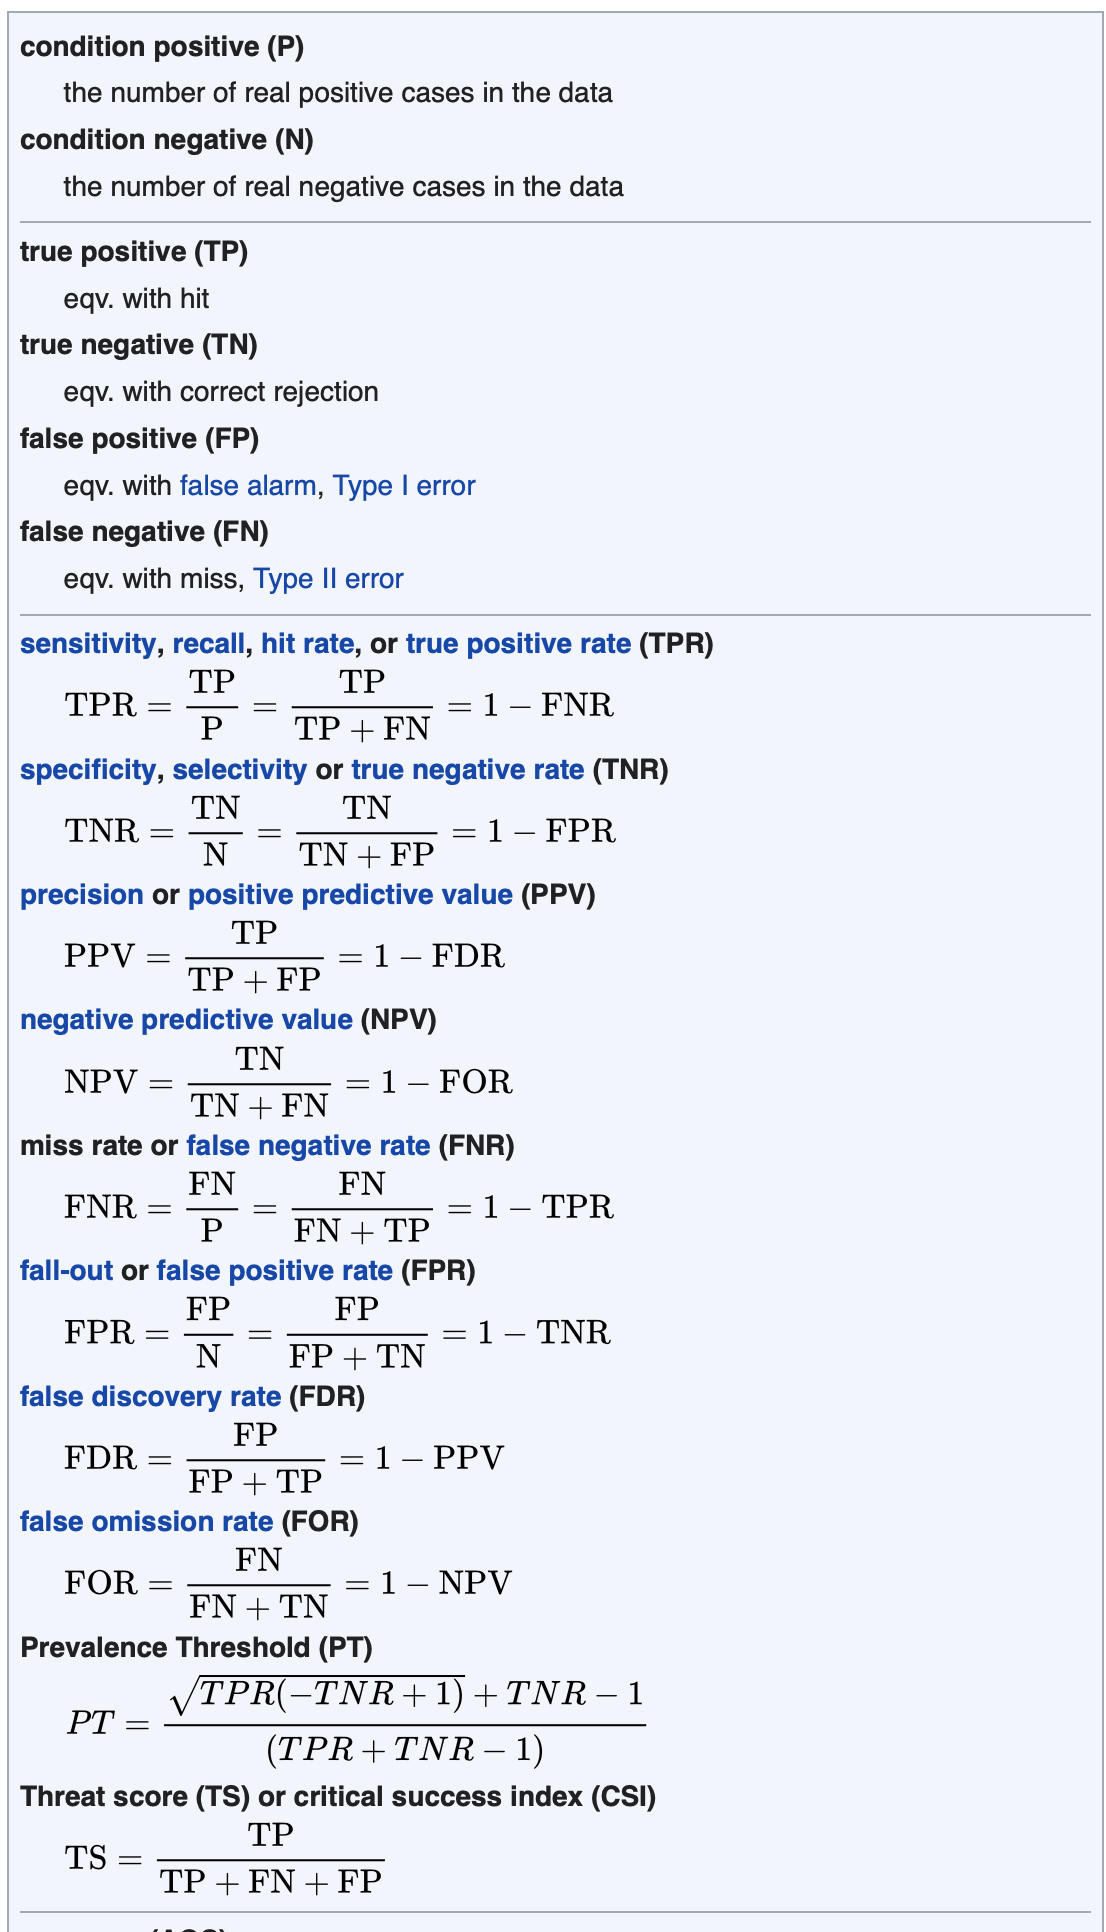
\includegraphics{../images/wiki-sensitivity.png}
\caption{Testing terms}
\end{figure}
\end{frame}

\begin{frame}{How To Solve These Problems}
\protect\hypertarget{how-to-solve-these-problems}{}
\begin{itemize}
\tightlist
\item
  Start with a table with the states of the world on one axis, and
  states of the test on the other axis.
\item
  In this case it can just be a 2*2 table.
\item
  In each cell, write down the initial probability of ending up in that
  cell.
\item
  That will be the probability of being in that state, times the
  probability of that test result given that you are in that state.
\item
  The formula we are constantly using here is
  \(Pr(A \wedge B) = Pr(A) Pr(B | A)\).
\end{itemize}
\end{frame}

\begin{frame}{The Table}
\protect\hypertarget{the-table}{}
\begin{longtable}[]{@{}lll@{}}
\toprule
& Test Positive & Test Negative \\
\midrule
\endhead
Have Disease & 0.027 & 0.003 \\
No Disease & 0.0485 & 0.9215 \\
\bottomrule
\end{longtable}

\(\pause\)

Let's talk for a bit about how we generated it.
\end{frame}

\begin{frame}{The Table}
\protect\hypertarget{the-table-1}{}
\begin{longtable}[]{@{}rcc@{}}
\toprule
& Test Positive & Test Negative \\
\midrule
\endhead
Have Disease & 0.027 & 0.003 \\
No Disease & 0.0485 & 0.9215 \\
\bottomrule
\end{longtable}

\begin{itemize}
\tightlist
\item
  Focus on the top left cell. Why does it say 0.027?
\item
  Well, probability of disease is, we said, 0.03.
\item
  And probability of test positive given disease is 0.9.
\item
  So probability of disease and test positive is 0.03 * 0.9 = 0.027, or
  2.7\%.
\end{itemize}
\end{frame}

\begin{frame}{The Table}
\protect\hypertarget{the-table-2}{}
\begin{longtable}[]{@{}rcc@{}}
\toprule
& Test Positive & Test Negative \\
\midrule
\endhead
Have Disease & 0.027 & 0.003 \\
No Disease & 0.0485 & 0.9215 \\
\bottomrule
\end{longtable}

\begin{itemize}
\tightlist
\item
  Now focus on the top right cell. Why does it say 0.003?
\item
  Well, probability of disease is, we said, 0.03.
\item
  And probability of test negative given disease is 1 - 0.9, i.e., 0.1.
\item
  So probability of disease and test positive is 0.03 * 0.1 = 0.003, or
  0.3\%.
\end{itemize}
\end{frame}

\begin{frame}{The Table}
\protect\hypertarget{the-table-3}{}
\begin{longtable}[]{@{}rcc@{}}
\toprule
& Test Positive & Test Negative \\
\midrule
\endhead
Have Disease & 0.027 & 0.003 \\
No Disease & 0.0485 & 0.9215 \\
\bottomrule
\end{longtable}

\begin{itemize}
\tightlist
\item
  Now focus on the bottom left cell. Why does it say 0.0485?
\item
  Well, probability of disease is, we said, 0.03.
\item
  So probability of non-disease is 0.97.
\item
  And probability of test positive given non-disease is 0.05.
\item
  So probability of non-disease and test positive is 0.97 * 0.05 =
  0.0485, or 4.85\%.
\end{itemize}
\end{frame}

\begin{frame}{The Table}
\protect\hypertarget{the-table-4}{}
\begin{longtable}[]{@{}rcc@{}}
\toprule
& Test Positive & Test Negative \\
\midrule
\endhead
Have Disease & 0.027 & 0.003 \\
No Disease & 0.0485 & 0.9215 \\
\bottomrule
\end{longtable}

\begin{itemize}
\tightlist
\item
  Now focus on the bottom right cell. Why does it say 0.9215?
\item
  Well, probability of non-disease is 0.97.
\item
  And probability of test negative given non-disease is 1 - 0.05 = 0.95.
\item
  So probability of non-disease and test positive is 0.97 * 0.95 =
  0.9215, or 92.15\%.
\end{itemize}
\end{frame}

\begin{frame}{Solving the Problem}
\protect\hypertarget{solving-the-problem}{}
\begin{longtable}[]{@{}rcc@{}}
\toprule
& Test Positive & Test Negative \\
\midrule
\endhead
Have Disease & 0.027 & 0.003 \\
No Disease & 0.0485 & 0.9215 \\
\bottomrule
\end{longtable}

\begin{itemize}
\tightlist
\item
  We want to know Pr(Disease \(|\) Test Positive). Call this
  \(Pr(D | TP)\).\(\pause\)
\item
  That's \(Pr(D \wedge TP)\) divided by \(Pr(TP)\).\(\pause\)
\item
  And \(Pr(D \wedge TP)\) is 0.027.\(\pause\)
\item
  And \(Pr(TP)\) is 0.0755.\(\pause\)
\item
  So the answer is roughly 0.35, i.e., \(\frac{0.027}{0.0755}\).
\end{itemize}
\end{frame}

\begin{frame}{Practical Consequence}
\protect\hypertarget{practical-consequence}{}
\begin{itemize}
\tightlist
\item
  That test looked pretty reliable.
\item
  But testing positive only raises the probability of having the disease
  toa bit over 1 in 3.
\item
  This wasn't really a quirk of the example.
\item
  When testing for relatively rare conditions, this is a really common
  situation.
\item
  Unless the test is \textbf{really} reliable, testing positive is
  worrying, but usually raises the dreaded probability to well under 1,
  often under 0.5.
\end{itemize}
\end{frame}

\begin{frame}{General Strategy For A/B Problems}
\protect\hypertarget{general-strategy-for-ab-problems}{}
\begin{itemize}
\tightlist
\item
  Make a 2 x 2 table, with \(A, \neg A\) on the rows, and \(B, \neg B\)
  on the columns.
\item
  Work out the probability of each cell.
\item
  To do this, repeatedly use the formula
\end{itemize}

\[
\Pr(X \wedge Y) = \Pr(X | Y)\Pr(Y)
\]

\begin{itemize}
\tightlist
\item
  Add up the values across the rows to get \(\Pr(A), \Pr(\neg A)\).
\item
  Add up the values down the columns to get \(\Pr(B), \Pr(\neg B)\).
\item
  Use the formula for conditional probability to work out the answer.
\end{itemize}
\end{frame}

\begin{frame}{Another Example}
\protect\hypertarget{another-example}{}
\begin{itemize}
\tightlist
\item
  \(\Pr(A) = 0.6\).
\item
  \(\Pr(B | A) = 0.3\).
\item
  \(\Pr(B | \neg A) = 0.8\).
\item
  Find \(\Pr(B)\) and \(\Pr(A | B)\).
\end{itemize}
\end{frame}

\begin{frame}{Use the Negation Rule to fill in the Basic Probabilities}
\protect\hypertarget{use-the-negation-rule-to-fill-in-the-basic-probabilities}{}
\begin{itemize}
\tightlist
\item
  \(\Pr(A) = 0.6\), so \(\Pr(\neg A) = 0.4\). \pause
\item
  \(\Pr(B | A) = 0.3\), so \(\Pr(\neg B | A) = 0.7\). \pause
\item
  \(\Pr(B | \neg A) = 0.8\), sp \(\Pr(\neg B | \neg A) = 0.2\).
\end{itemize}
\end{frame}

\begin{frame}{Build the Table}
\protect\hypertarget{build-the-table}{}
\begin{longtable}[]{@{}rcc@{}}
\toprule
& \(B\) & \(\neg B\) \\
\midrule
\endhead
\(A\) & & \\
\(\neg A\) & & \\
\bottomrule
\end{longtable}
\end{frame}

\begin{frame}{Top Left Corner}
\protect\hypertarget{top-left-corner}{}
\begin{align*}
\Pr(A \wedge B) &= \Pr(B | A) \Pr(A) \\
 &= 0.3 \times 0.6 \\
 &= 0.18
\end{align*}

\pause

\begin{longtable}[]{@{}rcc@{}}
\toprule
& \(B\) & \(\neg B\) \\
\midrule
\endhead
\(A\) & 0.18 & \\
\(\neg A\) & & \\
\bottomrule
\end{longtable}
\end{frame}

\begin{frame}{Top Right Corner}
\protect\hypertarget{top-right-corner}{}
\begin{align*}
\Pr(A \wedge \neg B) &= \Pr(\neg B | A) \Pr(A) \\
 &= 0.7 \times 0.6 \\
 &= 0.42
\end{align*}

\pause

\begin{longtable}[]{@{}rcc@{}}
\toprule
& \(B\) & \(\neg B\) \\
\midrule
\endhead
\(A\) & 0.18 & 0.42 \\
\(\neg A\) & & \\
\bottomrule
\end{longtable}
\end{frame}

\begin{frame}{Check}
\protect\hypertarget{check}{}
\begin{longtable}[]{@{}rcc@{}}
\toprule
& \(B\) & \(\neg B\) \\
\midrule
\endhead
\(A\) & 0.18 & 0.42 \\
\(\neg A\) & & \\
\bottomrule
\end{longtable}

The numbers in the top row are 0.18 + 0.42 = 0.6, which is what we were
told \(\Pr(A)\) was. So our work passes this little cross-check.
\end{frame}

\begin{frame}{Bottom Left Corner}
\protect\hypertarget{bottom-left-corner}{}
\begin{align*}
\Pr(\neg A \wedge B) &= \Pr( B | \neg A) \Pr(\neg A) \\
 &= 0.8 \times 0.4 \\
 &= 0.32
\end{align*}

\pause

\begin{longtable}[]{@{}rcc@{}}
\toprule
& \(B\) & \(\neg B\) \\
\midrule
\endhead
\(A\) & 0.18 & 0.42 \\
\(\neg A\) & 0.32 & \\
\bottomrule
\end{longtable}
\end{frame}

\begin{frame}{Bottom Right Corner}
\protect\hypertarget{bottom-right-corner}{}
\begin{align*}
\Pr(\neg A \wedge \neg B) &= \Pr( \neg B | \neg A) \Pr(\neg A) \\
 &= 0.2 \times 0.4 \\
 &= 0.08
\end{align*}

\pause

\begin{longtable}[]{@{}rcc@{}}
\toprule
& \(B\) & \(\neg B\) \\
\midrule
\endhead
\(A\) & 0.18 & 0.42 \\
\(\neg A\) & 0.32 & 0.08 \\
\bottomrule
\end{longtable}
\end{frame}

\begin{frame}{Check}
\protect\hypertarget{check-1}{}
\begin{longtable}[]{@{}rcc@{}}
\toprule
& \(B\) & \(\neg B\) \\
\midrule
\endhead
\(A\) & 0.18 & 0.42 \\
\(\neg A\) & 0.32 & 0.08 \\
\bottomrule
\end{longtable}

\begin{itemize}
\tightlist
\item
  The bottom row sums to 0.4, as we knew \(\Pr(\neg A)\) was.
\item
  And the whole thing sums to 1, which is good.
\end{itemize}
\end{frame}

\begin{frame}{\(\Pr(B)\)}
\protect\hypertarget{prb}{}
\begin{longtable}[]{@{}rcc@{}}
\toprule
& \(B\) & \(\neg B\) \\
\midrule
\endhead
\(A\) & 0.18 & 0.42 \\
\(\neg A\) & 0.32 & 0.08 \\
\bottomrule
\end{longtable}

\begin{itemize}
\tightlist
\item
  \(\Pr(B) = 0.18 + 0.32 = 0.5\). \pause
\item
  \(\Pr(\neg B) = 0.42 + 0.08 = 0.5\) \pause
\item
  Given \(\Pr(B)\) we could have used the negation rule to work out
  \(\Pr(\neg B)\).
\end{itemize}
\end{frame}

\begin{frame}{\(\Pr(A | B)\)}
\protect\hypertarget{pra-b}{}
\begin{align*}
\Pr(A | B) &= \frac{\Pr(A \wedge B)}{\Pr(B)} \\
 &= \frac{0.18}{0.5} \\
 &= 0.36
\end{align*}

\begin{itemize}
\tightlist
\item
  So the answer is that \(\Pr(A | B)\) is 0.36.
\item
  If you learn \(B\), the probability of \(A\) falls from 0.6 to 0.36.
\end{itemize}
\end{frame}

\begin{frame}{For Next Time}
\protect\hypertarget{for-next-time}{}
\begin{itemize}
\tightlist
\item
  We will revise the rules of probability, with special focus on the
  rules that you use to solve these kinds of problems.
\end{itemize}
\end{frame}

\end{document}
